\documentclass[11pt,preprint, authoryear]{elsarticle}

\usepackage{lmodern}
%%%% My spacing
\usepackage{setspace}
\setstretch{1.2}
\DeclareMathSizes{12}{14}{10}{10}

% Wrap around which gives all figures included the [H] command, or places it "here". This can be tedious to code in Rmarkdown.
\usepackage{float}
\let\origfigure\figure
\let\endorigfigure\endfigure
\renewenvironment{figure}[1][2] {
    \expandafter\origfigure\expandafter[H]
} {
    \endorigfigure
}

\let\origtable\table
\let\endorigtable\endtable
\renewenvironment{table}[1][2] {
    \expandafter\origtable\expandafter[H]
} {
    \endorigtable
}


\usepackage{ifxetex,ifluatex}
\usepackage{fixltx2e} % provides \textsubscript
\ifnum 0\ifxetex 1\fi\ifluatex 1\fi=0 % if pdftex
  \usepackage[T1]{fontenc}
  \usepackage[utf8]{inputenc}
\else % if luatex or xelatex
  \ifxetex
    \usepackage{mathspec}
    \usepackage{xltxtra,xunicode}
  \else
    \usepackage{fontspec}
  \fi
  \defaultfontfeatures{Mapping=tex-text,Scale=MatchLowercase}
  \newcommand{\euro}{€}
\fi

\usepackage{amssymb, amsmath, amsthm, amsfonts}

\def\bibsection{\section*{References}} %%% Make "References" appear before bibliography


\usepackage[round]{natbib}

\usepackage{longtable}
\usepackage[margin=2.3cm,bottom=2cm,top=2.5cm, includefoot]{geometry}
\usepackage{fancyhdr}
\usepackage[bottom, hang, flushmargin]{footmisc}
\usepackage{graphicx}
\numberwithin{equation}{section}
\numberwithin{figure}{section}
\numberwithin{table}{section}
\setlength{\parindent}{0cm}
\setlength{\parskip}{1.3ex plus 0.5ex minus 0.3ex}
\usepackage{textcomp}
\renewcommand{\headrulewidth}{0.2pt}
\renewcommand{\footrulewidth}{0.3pt}

\usepackage{array}
\newcolumntype{x}[1]{>{\centering\arraybackslash\hspace{0pt}}p{#1}}

%%%%  Remove the "preprint submitted to" part. Don't worry about this either, it just looks better without it:
\makeatletter
\def\ps@pprintTitle{%
  \let\@oddhead\@empty
  \let\@evenhead\@empty
  \let\@oddfoot\@empty
  \let\@evenfoot\@oddfoot
}
\makeatother

 \def\tightlist{} % This allows for subbullets!

\usepackage{hyperref}
\hypersetup{breaklinks=true,
            bookmarks=true,
            colorlinks=true,
            citecolor=blue,
            urlcolor=blue,
            linkcolor=blue,
            pdfborder={0 0 0}}


% The following packages allow huxtable to work:
\usepackage{siunitx}
\usepackage{multirow}
\usepackage{hhline}
\usepackage{calc}
\usepackage{tabularx}
\usepackage{booktabs}
\usepackage{caption}


\newenvironment{columns}[1][]{}{}

\newenvironment{column}[1]{\begin{minipage}{#1}\ignorespaces}{%
\end{minipage}
\ifhmode\unskip\fi
\aftergroup\useignorespacesandallpars}

\def\useignorespacesandallpars#1\ignorespaces\fi{%
#1\fi\ignorespacesandallpars}

\makeatletter
\def\ignorespacesandallpars{%
  \@ifnextchar\par
    {\expandafter\ignorespacesandallpars\@gobble}%
    {}%
}
\makeatother

\newlength{\cslhangindent}
\setlength{\cslhangindent}{1.5em}
\newenvironment{CSLReferences}%
  {\setlength{\parindent}{0pt}%
  \everypar{\setlength{\hangindent}{\cslhangindent}}\ignorespaces}%
  {\par}


\urlstyle{same}  % don't use monospace font for urls
\setlength{\parindent}{0pt}
\setlength{\parskip}{6pt plus 2pt minus 1pt}
\setlength{\emergencystretch}{3em}  % prevent overfull lines
\setcounter{secnumdepth}{5}

%%% Use protect on footnotes to avoid problems with footnotes in titles
\let\rmarkdownfootnote\footnote%
\def\footnote{\protect\rmarkdownfootnote}
\IfFileExists{upquote.sty}{\usepackage{upquote}}{}

%%% Include extra packages specified by user
\usepackage{colortbl}
\usepackage{xcolor}

%%% Hard setting column skips for reports - this ensures greater consistency and control over the length settings in the document.
%% page layout
%% paragraphs
\setlength{\baselineskip}{12pt plus 0pt minus 0pt}
\setlength{\parskip}{12pt plus 0pt minus 0pt}
\setlength{\parindent}{0pt plus 0pt minus 0pt}
%% floats
\setlength{\floatsep}{12pt plus 0 pt minus 0pt}
\setlength{\textfloatsep}{20pt plus 0pt minus 0pt}
\setlength{\intextsep}{14pt plus 0pt minus 0pt}
\setlength{\dbltextfloatsep}{20pt plus 0pt minus 0pt}
\setlength{\dblfloatsep}{14pt plus 0pt minus 0pt}
%% maths
\setlength{\abovedisplayskip}{12pt plus 0pt minus 0pt}
\setlength{\belowdisplayskip}{12pt plus 0pt minus 0pt}
%% lists
\setlength{\topsep}{10pt plus 0pt minus 0pt}
\setlength{\partopsep}{3pt plus 0pt minus 0pt}
\setlength{\itemsep}{5pt plus 0pt minus 0pt}
\setlength{\labelsep}{8mm plus 0mm minus 0mm}
\setlength{\parsep}{\the\parskip}
\setlength{\listparindent}{\the\parindent}
%% verbatim
\setlength{\fboxsep}{5pt plus 0pt minus 0pt}



\begin{document}



\begin{frontmatter}  %

\title{Exploring Risk and Uncertainty in the Local Equity Market}

% Set to FALSE if wanting to remove title (for submission)




\author[Add1]{24693197}
\ead{24693197@sun.ac.za}





\address[Add1]{Stellenbosch University, Stellenbosch, South Africa}


\begin{abstract}
\small{
Abstract to be written here. The abstract should not be too long and
should provide the reader with a good understanding what you are writing
about. Academic papers are not like novels where you keep the reader in
suspense. To be effective in getting others to read your paper, be as
open and concise about your findings here as possible. Ideally, upon
reading your abstract, the reader should feel he / she must read your
paper in entirety.
}
\end{abstract}

\vspace{1cm}


\begin{keyword}
\footnotesize{
Multivariate GARCH \sep Kalman Filter \sep Copula \\
\vspace{0.3cm}
}
\footnotesize{
\textit{JEL classification} L250 \sep L100
}
\end{keyword}



\vspace{0.5cm}

\end{frontmatter}



%________________________
% Header and Footers
%%%%%%%%%%%%%%%%%%%%%%%%%%%%%%%%%
\pagestyle{fancy}
\chead{}
\rhead{}
\lfoot{}
\rfoot{\footnotesize Page \thepage}
\lhead{}
%\rfoot{\footnotesize Page \thepage } % "e.g. Page 2"
\cfoot{}

%\setlength\headheight{30pt}
%%%%%%%%%%%%%%%%%%%%%%%%%%%%%%%%%
%________________________

\headsep 35pt % So that header does not go over title




\section{\texorpdfstring{Introduction
\label{Introduction}}{Introduction }}\label{introduction}

This report will look at how offshore economic and policy uncertainty
affects the local equity market, and whether local funds need more
protection against volatility. Part A will establish whether local
volatility has increased and whether it follows global markets. Part B
will evaluate whether SafeCore has navigated volatility effectively,
where its volatility comes from and what its factor exposures are. Part
C will look at the alpha opportunity in the local market since 2020 and
how it changes with global policy uncertainty.

\section{\texorpdfstring{Part A: \label{PartA}}{Part A: }}\label{part-a}

\subsection{Data and approach}\label{data-and-approach}

This section will look at whether volatility on the local stock exchange
has increased and whether it follows global markets. Volatility refers
to how much returns of an asset deviates from its average and is
measured as the standard deviation (of daily returns). It is annualised
by multiplying it by the square root of 252, which is the approximate
number of trading days in a year, so that the figures are easier to
compare.

The local market is represented by the Capped SWIX (J433), which is the
broad market index and the fund's benchmark, together with the Mid Cap
(J201) and Small Cap (J202) indexes. Including the size indexes shows
whether changes in volatility are limited to the largest companies or
are present across the market. Global markets are represented by MSCI
World, which covers developed markets, and MSCI Emerging Markets (South
Africa is typically grouped with other emerging markets by global
investors). The comparison starts in 2015 as this is the first date of
the local data. The MSCI indexes are in USD and the local indexes in
ZAR, so naturally part of any difference in levels is due to currency
movements.

\subsection{Volatility over time}\label{volatility-over-time}

The first measure is a rolling standard deviation. For each day, the
standard deviation is calculated over the previous 63 trading days and
the window then moves forward one day at a time. A 63 day window
(roughly three months) was chosen as it reacts to changes in the market
without being too noisy. It also matches the three month horizon of the
SAVIUSD currency volatility index.

\begin{figure}[H]

{\centering \includegraphics{Question1_files/figure-latex/Figure_RollVol-1} 

}

\caption{Rolling 3 month annualised volatility: local vs global equity \label{Figure_RollVol}}\label{fig:Figure_RollVol}
\end{figure}

Figure \ref{Figure_RollVol} shows that local and global volatility both
have the largest increases happening at the same time, thus they tend to
move closely together. In 2020 and in 2025, local and global volatility
increased together (and by a similar amount). This suggests that local
markets are affected by shocks that start offshore. In the most recent
period, local volatility has increased together with emerging market
volatility and developed market volatility has stayed low.

\subsection{Has volatility increased?}\label{has-volatility-increased}

As the rolling measure can be difficult to read over a long period,
Figure \ref{Figure_AnnVol} summarises volatility by calendar year
instead.

\begin{figure}[H]

{\centering \includegraphics{Question1_files/figure-latex/Figure_AnnVol-1} 

}

\caption{Calendar year realised volatility \label{Figure_AnnVol}}\label{fig:Figure_AnnVol}
\end{figure}

Figure \ref{Figure_AnnVol} shows that local volatility has not increased
steadily over time. Instead, it increases in ceratin episodes. There are
clear peaks in 2020, 2022 and 2026. Apart from 2020, Capped SWIX
volatility in 2026 is the highest since 2015, although the 2026 figure
only includes data up to September. Mid and small cap volatility has
stayed above its pre-2020 level since 2021, which suggests that the
increase is not limited to the largest companies. Local volatility is
also higher than MSCI World in almost every year and closer to MSCI
Emerging Markets. In 2026, volatility rose again across all of the
series considered. The increase was most pronounced for emerging
markets, while developed market volatility rose by less. Local
volatility followed this increase, although to a lesser extent than
emerging markets as a group.

\subsection{Separating the volatility signal from
noise}\label{separating-the-volatility-signal-from-noise}

A limitation of the rolling standard deviation is that it is noisy, as a
single extreme day affects the estimate for the whole window. A GARCH
model addresses this by separating returns into an underlying level of
volatility, called sigma, and random day-to-day noise. It does this by
using the fact that volatility tends to cluster, meaning that a volatile
day is usually followed by another volatile day.

This section uses a GJR-GARCH model, which allows negative returns to
increase volatility by more than positive returns of the same size (the
leverage effect). This was chosen as the standard GARCH model treats
positive and negative shocks the same, while in practice negative
returns in stock markets tend to raise volatility by more than positive
returns. The model is fitted to the Capped SWIX and MSCI World
separately.

\begin{figure}[H]

{\centering \includegraphics{Question1_files/figure-latex/Figure_Garch-1} 

}

\caption{GJR-GARCH conditional volatility: Capped SWIX vs MSCI World \label{Figure_Garch}}\label{fig:Figure_Garch}
\end{figure}

Figure \ref{Figure_Garch} shows that the large increases in global
volatility, such as in 2018, 2020, 2022 and 2025, line up with increases
in local volatility. This suggests that local markets follow global
markets during periods of stress. Global volatility increases more
sharply during these episodes. In calmer periods local volatility
remains higher than that of developed markets. The 2026 increase is
different, as local volatility rose while developed market volatility
stayed low. This matches the emerging market pattern in Figures
\ref{Figure_RollVol} and \ref{Figure_AnnVol}.

\begin{table}[H]
\centering
\begin{tabular}{rrrrr}
  \hline
 &  Estimate &  Std. Error &  t value & Pr($>$$|$t$|$) \\ 
  \hline
mu & 0.0004 & 0.0002 & 2.7333 & 0.0063 \\ 
  ar1 & 0.0009 & 0.0185 & 0.0502 & 0.9599 \\ 
  omega & 0.0000 & 0.0000 & 3.4435 & 0.0006 \\ 
  alpha1 & 0.0043 & 0.0040 & 1.0707 & 0.2843 \\ 
  beta1 & 0.8997 & 0.0096 & 94.1836 & 0.0000 \\ 
  gamma1 & 0.1288 & 0.0180 & 7.1677 & 0.0000 \\ 
  shape & 6.7905 & 0.7356 & 9.2314 & 0.0000 \\ 
   \hline
\end{tabular}
\caption{GJR-GARCH(1,1) estimates: Capped SWIX \label{Table_Garch_J433}} 
\end{table}
\begin{table}[H]
\centering
\begin{tabular}{rrrrr}
  \hline
 &  Estimate &  Std. Error &  t value & Pr($>$$|$t$|$) \\ 
  \hline
mu & 0.0006 & 0.0001 & 5.1461 & 0.0000 \\ 
  ar1 & 0.0834 & 0.0182 & 4.5774 & 0.0000 \\ 
  omega & 0.0000 & 0.0000 & 1.6317 & 0.1027 \\ 
  alpha1 & 0.0002 & 0.0117 & 0.0140 & 0.9888 \\ 
  beta1 & 0.8633 & 0.0160 & 53.8728 & 0.0000 \\ 
  gamma1 & 0.2349 & 0.0363 & 6.4727 & 0.0000 \\ 
  shape & 6.0507 & 0.6357 & 9.5186 & 0.0000 \\ 
   \hline
\end{tabular}
\caption{GJR-GARCH(1,1) estimates: MSCI World \label{Table_Garch_MXWO}} 
\end{table}

Tables \ref{Table_Garch_J433} and \ref{Table_Garch_MXWO} report the
estimated parameters of the model. The parameter alpha1 measures how
much volatility reacts to any new shock, gamma1 measures the extra
reaction to negative shocks, and beta1 measures how much of yesterday's
volatility carries over to today. Persistence combines these and shows
how slowly a volatility shock fades, where values close to one mean that
shocks fade slowly.

For both indexes, alpha1 is close to zero while gamma1 is large,
although the p-values of a GARCH fit should not be interpreted too
strictly. Therefore, volatility increases mainly after negative returns
rather than after positive ones. This effect is stronger for MSCI World,
which is consistent with the sharper global spikes in Figure
\ref{Figure_Garch}. Persistence is close to one for both indexes, at
0.968 for the Capped SWIX and 0.981 for MSCI World, so once volatility
increases in either market it takes a long time to settle.

\subsection{Summary}\label{summary}

In summary, local volatility has not increased steadily. It does seem to
increase sharply when offshore shocks hit, and these shocks are then
passed on to the local market. The most recent rise in volatility in
2026 was broad-based, but was strongest in emerging markets. This means
that local funds remain exposed to offshore uncertainty.

\section{Part B:}\label{part-b}

This section will look at whether SafeCore has handled volatility well.
As volatility is not explicitly considered when SafeCore is constructed,
its lack of a low volatility tilt is not surprising. However, the
results show that the fund does not avoid volatility by chance either.
It is concentrated in volatile resource stocks and leans towards recent
winners, which supports the concern raised by colleagues. SafeCore only
reports its monthly holdings, so its daily returns are calculated by
applying the monthly weights to the daily returns of the stocks it
holds. The Capped SWIX is used as the benchmark throughout.

\begin{figure}[H]

{\centering \includegraphics{Question1_files/figure-latex/Figure_SafeCore_Cum-1} 

}

\caption{Cumulative returns: SafeCore vs Capped SWIX \label{Figure_SafeCore_Cum}}\label{fig:Figure_SafeCore_Cum}
\end{figure}

Figure \ref{Figure_SafeCore_Cum} shows that SafeCore has outperformed
its benchmark since 2015, ending the period well above the Capped SWIX.

\begin{table}[H]
\centering
\begin{tabular}{llrr}
  \hline
Period & Info & SafeCore & J433 \\ 
  \hline
Last 3 Years & Cum Returns & 0.760 & 0.696 \\ 
  Last 3 Years & Returns (Ann.) & 0.207 & 0.193 \\ 
  Last 3 Years & Returns Excess (Ann.) & 0.012 & 0.000 \\ 
  Last 3 Years & SD (Ann.) & 0.134 & 0.128 \\ 
  Last 3 Years & Adj. Sharpe Ratio & 1.157 & 0.853 \\ 
  Last 3 Years & Pain Index & 0.028 & 0.026 \\ 
  Last 3 Years & Avg DD & 0.061 & 0.047 \\ 
  Last 3 Years & Tracking Error & 0.032 & 0.000 \\ 
  Last 3 Years & Information Ratio & 0.460 &  \\ 
  Last 3 Years & Beta & 1.018 & 1.000 \\ 
  Last 3 Years & Beta Bull & 1.072 & 1.000 \\ 
  Last 3 Years & Beta Bear & 0.838 & 1.000 \\ 
  Last 3 Years & Up-Down Ratio & 0.680 & 0.000 \\ 
  Last 3 Years & Modified CVaR & -0.076 & -0.083 \\ 
  Last 5 Years & Cum Returns & 0.977 & 0.919 \\ 
  Last 5 Years & Returns (Ann.) & 0.146 & 0.139 \\ 
  Last 5 Years & Returns Excess (Ann.) & 0.006 & 0.000 \\ 
  Last 5 Years & SD (Ann.) & 0.148 & 0.137 \\ 
  Last 5 Years & Adj. Sharpe Ratio & 0.933 & 0.918 \\ 
  Last 5 Years & Pain Index & 0.040 & 0.032 \\ 
  Last 5 Years & Avg DD & 0.098 & 0.069 \\ 
  Last 5 Years & Tracking Error & 0.035 & 0.000 \\ 
  Last 5 Years & Information Ratio & 0.193 &  \\ 
  Last 5 Years & Beta & 1.053 & 1.000 \\ 
  Last 5 Years & Beta Bull & 0.997 & 1.000 \\ 
  Last 5 Years & Beta Bear & 0.905 & 1.000 \\ 
  Last 5 Years & Up-Down Ratio & 0.615 & 0.000 \\ 
  Last 5 Years & Modified CVaR & -0.081 & -0.079 \\ 
   \hline
\end{tabular}
\caption{SafeCore statistics relative to the Capped SWIX \label{Table_Stats}} 
\end{table}

Table \ref{Table_Stats} compares SafeCore to the Capped SWIX over the
last three and five years. These periods were chosen to focus on the
fund's recent behaviour. SafeCore has outperformed over both periods,
but with higher volatility than its benchmark.

The drawdown measures show how far the fund falls from a previous peak.
Over five years, SafeCore's average drawdown is 9.8\%, while that of the
Capped SWIX is 6.9\%, so when SafeCore falls, it tends to fall further.
Its bear beta, which measures how the fund moves in months when the
benchmark falls, is below one. This suggests that SafeCore is affected
less by market declines in a normal down month but suffers larger
declines when the market falls over a longer period.

SafeCore also has a higher adjusted Sharpe ratio over three years. The
Sharpe ratio measures the return earned per unit of volatility. This
means SafeCore has been rewarded for its risk, but it has still taken on
more risk than its benchmark in recent years.

\begin{table}[H]
\centering
\begin{tabular}{rrr}
  \hline
 & SafeCore & J433 \\ 
  \hline
Semi Deviation & 0.0078 & 0.0081 \\ 
  Downside Deviation (Rf=0\%) & 0.0076 & 0.0080 \\ 
  Maximum Drawdown & 0.3765 & 0.4166 \\ 
  Historical VaR (95\%) & -0.0163 & -0.0165 \\ 
  Historical ES (95\%) & -0.0244 & -0.0257 \\ 
  Modified VaR (95\%) & -0.0175 & -0.0179 \\ 
  Modified ES (95\%) & -0.0310 & -0.0349 \\ 
   \hline
\end{tabular}
\caption{Downside risk measures: SafeCore vs Capped SWIX \label{Table_Downside}} 
\end{table}

The downside risk measures only consider losses, which is what matters
most when volatility increases. Semi-deviation and downside deviation
measure the volatility of returns below the mean and below zero. Value
at Risk (VaR) is the loss that is exceeded on only 5\% of days, and
Expected Shortfall (ES) is the average loss on those worst days. Over
the full period since 2015, SafeCore has lower downside risk than the
Capped SWIX on every measure. For example, its maximum drawdown is
37.7\%, while that of the Capped SWIX is 41.7\%.

\begin{figure}[H]

{\centering \includegraphics{Question1_files/figure-latex/Figure_Drawdown-1} 

}

\caption{SafeCore drawdown relative to the Capped SWIX \label{Figure_Drawdown}}\label{fig:Figure_Drawdown}
\end{figure}

The full-period result and the recent three and five year results point
in different directions, so Figure \ref{Figure_Drawdown} looks at how
this changed over time. It plots the difference between SafeCore's
drawdown and that of the Capped SWIX, where positive values mean
SafeCore fell less. SafeCore's advantage was mainly between 2015 and
2017 and in 2020. Since 2021, the difference has been close to zero or
negative, especially in 2022. Therefore, SafeCore's protection on the
downside has weakened in recent years, at the same time as offshore
volatility has increased.

In summary, SafeCore has delivered strong returns, but the protection it
offered in earlier years has weakened just as offshore volatility has
increased. The next section therefore looks at where SafeCore's risk
comes from.

\subsection{Sources of SafeCore's
volatility}\label{sources-of-safecores-volatility}

\begin{figure}[H]

{\centering \includegraphics{Question1_files/figure-latex/Figure_Risk-1} 

}

\caption{SafeCore weight and risk contribution by sector \label{Figure_Risk}}\label{fig:Figure_Risk}
\end{figure}

To understand where SafeCore's volatility comes from, Figure
\ref{Figure_Risk} compares the share of the fund held in each sector to
the share of the fund's volatility that each sector is responsible for.
This is based on the fund's average holdings and daily returns over the
last 12 months, which captures how the fund has been positioned over the
past year. The risk contribution is not the same as the weight, as it
also depends on how volatile each stock is and how closely it moves with
the rest of the fund. A sector whose risk share is above its weight
therefore adds more volatility than its size suggests.

The figure shows that SafeCore's volatility is concentrated in resource
stocks. Two holdings, Pan African Resources and Valterra Platinum, have
no sector in the fund data and were classified as resources using the
index constituent data. Resources make up just over a third of the fund
but are responsible for around two thirds of its volatility, while
financials and industrials add far less volatility than their weight.
Resource stocks depend on global commodity prices, which makes them
exposed to offshore shocks. Therefore, SafeCore's risk comes mainly from
the part of the fund that is most affected by the offshore volatility
identified in Part A.

\subsection{Factor exposures}\label{factor-exposures}

This section will construct a momentum and a low volatility score for
each stock using price behaviour only. For momentum, each stock's
cumulative return over the past six months is calculated, excluding the
most recent month. The most recent month is left out so that the score
reflects a more persistent trend rather than the latest short-term
movement. For low volatility, each stock's realised volatility is
calculated from the past six months of daily returns. A six month window
captures recent price behaviour while being long enough not to react
strongly to short-lived spikes. Since a lower volatility should
correspond to a higher low volatility score, the sign of the volatility
measure is reversed. Both measures are then standardised each month, so
that every stock's score is expressed relative to the other stocks at
that point in time. This places the scores on the same scale as the
third-party factor scores, which allows the two to be compared directly.

\begin{figure}[H]

{\centering \includegraphics{Question1_files/figure-latex/Figure_ScoreCor-1} 

}

\caption{Correlation between own and third-party factor scores \label{Figure_ScoreCor}}\label{fig:Figure_ScoreCor}
\end{figure}

To compare the scores, Figure \ref{Figure_ScoreCor} shows the
correlation between the own and third-party scores across all stocks in
each month. The own momentum score is closely related to the third-party
momentum score, with a correlation of between 0.6 and 0.85 in most
months. The main exception is early 2021, when the correlation fell
sharply. This suggests that the two scores measure different things.
Therefore, the own low volatility score provides information that is not
captured by the third-party scores.

The relationship between the own low volatility score and the
third-party volatility sensitivity score is weaker. A higher volatility
sensitivity score means a more volatile stock. This score was therefore
reversed, which means that a higher value indicates a less volatile
stock for both scores. Since late 2022, the correlation has been
positive in most months. This means that the two scores mostly agree on
which stocks are more volatile. However, the correlation is low and is
negative in some periods. Therefore, the two scores do not measure
exactly the same thing, and the own score adds information that the
third-party scores do not capture.

\begin{figure}[H]

{\centering \includegraphics{Question1_files/figure-latex/Figure_Composite-1} 

}

\caption{Composite factor scores: SafeCore, benchmark and strategy indexes \label{Figure_Composite}}\label{fig:Figure_Composite}
\end{figure}

To place SafeCore's factor exposures in context, Figure
\ref{Figure_Composite} shows the composite score of each portfolio,
calculated as the weighted average score of its holdings in August 2026.
All holdings had factor scores available, so the composite scores are
based on the full portfolios. A positive score means the portfolio leans
towards that factor, while a negative score means it leans away from it.
As a check, each strategy index scores highest on its own factor, and
the Capped SWIX sits close to zero on most factors. This is as expected
for the broad market.

The figure shows that SafeCore has a strong momentum tilt, with a
third-party momentum score as high as that of the Momentum index, while
the Capped SWIX is close to zero. SafeCore also leans slightly towards
value and earnings quality. However, it has no low volatility tilt, as
its own low volatility score is slightly below that of its benchmark.
Together with the results in Figure \ref{Figure_Risk}, this suggests
that SafeCore holds stocks that have performed well recently (many of
them resource stocks) without any defensive tilt to protect the fund
when the market turns.

\subsection{Summary}\label{summary-1}

In summary, SafeCore has outperformed its benchmark, but its protection
during market declines has weakened as offshore volatility has
increased. Its risk is concentrated in resource stocks, which are highly
exposed to offshore shocks, and its factor exposures show a strong
momentum tilt with no low volatility tilt. The team should be aware that
SafeCore's current positioning leaves it exposed to offshore shocks.

\section{Part C}\label{part-c}

\subsection{Dispersion}\label{dispersion}

\begin{figure}[H]

{\centering \includegraphics{Question1_files/figure-latex/Figure_Disp-1} 

}

\caption{Rolling dispersion of Capped SWIX constituents \label{Figure_Disp}}\label{fig:Figure_Disp}
\end{figure}

Cross-sectional volatility (dispersion) measures the average weighted
difference in returns between the constituents of an index and the
parent index itself. When dispersion is low, the opportunity for active
managers to differentiate their portfolios from the index is low, while
high dispersion indicates a greater opportunity to do so. This section
will calculate both weighted and unweighted dispersion for the Capped
SWIX constituents over a rolling three month window. The weighted
measure is used as the main measure, as SafeCore is managed against the
Capped SWIX and the weighted measure compares each stock to the index
return in line with its index weight. The unweighted measure is shown
for comparison. The constituent data starts in August 2020, so the
analysis covers the full period available since 2020.

Figure \ref{Figure_Disp} shows that dispersion is not constant, but
increases sharply in certain periods before returning to lower levels.
These periods of high dispersion represent the times when the
opportunity to differentiate a portfolio from the Capped SWIX was
greatest. The weighted measure is higher than the unweighted measure
during most of these periods, which indicates that the largest
constituents in particular moved apart from the index.

\subsection{Comovement between
constituents}\label{comovement-between-constituents}

This section will look at how the comovement between the constituents of
the Capped SWIX changes over time. The correlation coefficient measures
the linear dependence between two assets, and asset market correlations
typically increase in periods of turmoil, as turmoil leads to greater
homogeneity in asset prices. For each month, the correlation matrix of
the constituents' daily returns is calculated and the average
correlation across all pairs of stocks is taken.

\begin{figure}[H]

{\centering 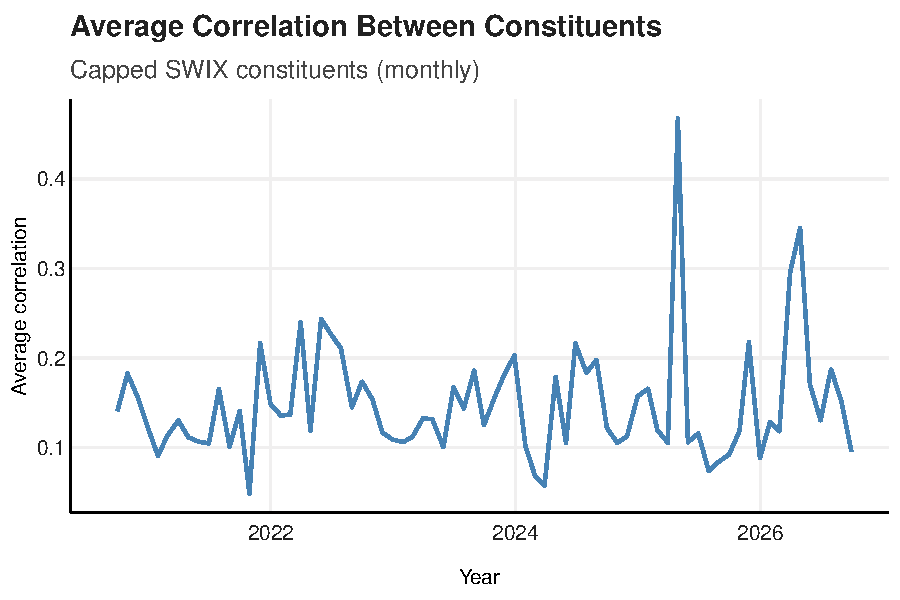
\includegraphics{Question1_files/figure-latex/Figure_Cor-1} 

}

\caption{Average correlation between Capped SWIX constituents \label{Figure_Cor}}\label{fig:Figure_Cor}
\end{figure}

Figure \ref{Figure_Cor} shows that the average correlation is generally
low, but increases in certain periods (most notably in 2025 and 2026).
Asset market correlations typically increase in periods of turmoil, as
turmoil leads to asset market price homogeneity. It should be noted that
a rolling correlation requires a look-back window and keeps the noise. A
DCC estimate would instead provide a cleaner, noise-reduced version of
the comovement structure between the constituents.

\subsection{Alpha opportunity and global
uncertainty}\label{alpha-opportunity-and-global-uncertainty}

This section will look at how the alpha opportunity has increased or
decreased with key global macro factors. As the seminar focused on
global policy uncertainty, the global economic policy uncertainty index
is used. The months are stratified into environments, where months in
which policy uncertainty is above its 85th percentile are classified as
high uncertainty, months below its 25th percentile as low uncertainty,
and the remaining months as other. The average weighted dispersion and
average correlation are then compared across these environments.

\begin{table}[H]
\centering
\begin{tabular}{lrr}
  \hline
Environment & Dispersion & Correlation \\ 
  \hline
High uncertainty & 0.164 & 0.173 \\ 
  Low uncertainty & 0.135 & 0.129 \\ 
  Other & 0.146 & 0.149 \\ 
   \hline
\end{tabular}
\caption{Average dispersion and correlation by level of global policy uncertainty \label{Table_Enviro}} 
\end{table}

Table \ref{Table_Enviro} shows that both dispersion and correlation are
higher in periods of high global policy uncertainty than in periods of
low uncertainty. The higher correlation is consistent with turmoil
leading to asset market price homogeneity. Since high dispersion means
that the alpha opportunity (the ability to differentiate portfolios) is
high, this suggests that the alpha opportunity in the local market has
increased with global policy uncertainty. As only a small number of
months fall into each environment, these results should be interpreted
with caution.

As the seminar also focused on oil price volatility, the same
stratification is repeated using the monthly volatility of Brent crude
oil, with the same percentile cut-offs.

\begin{figure}[H]

{\centering \includegraphics{Question1_files/figure-latex/Figure_Enviro-1} 

}

\caption{Dispersion and correlation by level of global policy uncertainty and oil price volatility \label{Figure_Enviro}}\label{fig:Figure_Enviro}
\end{figure}

Figure \ref{Figure_Enviro} compares both macro factors. For both global
policy uncertainty and oil price volatility, dispersion and correlation
increase from low to high months, and the increase in correlation is
larger for oil. The higher correlation is consistent with turmoil
leading to asset market price homogeneity. Since high dispersion means
that the alpha opportunity (the ability to differentiate portfolios) is
high, this suggests that the alpha opportunity in the local market has
increased with both global policy uncertainty and oil price volatility.

\subsection{Summary}\label{summary-2}

Overall, the results in Part C suggest that the alpha opportunity in the
local market since 2020 has not been constant, but has risen in
episodes. Dispersion between constituents rises sharply in certain
periods, and these periods tend to coincide with high global policy
uncertainty. Although stocks move together more closely during these
periods, the larger spread in their returns suggests that active
managers have had greater scope to differentiate their portfolios when
global uncertainty is high.

\section{Conclusion}\label{conclusion}

This report looked at how offshore uncertainty affects the local equity
market and SafeCore. Part A showed that local volatility is not much
higher than before, but is high in certain periods, mostly when offshore
shocks occur. Part B showed that SafeCore has outperformed its
benchmark, but its protection in down markets has weakened. Its
volatility comes mainly from resource stocks, and it has a momentum tilt
with no low volatility tilt. Part C showed that the alpha opportunity in
the local market has been greater when global policy uncertainty is
high. Therefore, SafeCore could benefit from more protection against
volatility, while still making use of the opportunities that come with
periods of high uncertainty.

\newpage

\section*{References}\label{references}
\addcontentsline{toc}{section}{References}

\protect\phantomsection\label{refs}

\section*{Appendix}\label{appendix}
\addcontentsline{toc}{section}{Appendix}

\subsection*{Appendix A}\label{appendix-a}
\addcontentsline{toc}{subsection}{Appendix A}

Some appendix information here

\subsection*{Appendix B}\label{appendix-b}
\addcontentsline{toc}{subsection}{Appendix B}

\bibliography{Tex/ref}





\end{document}
